\chapter{Modelagem geral do sistema}

Tendo esclarecido sobre as questões gerais do trabalho e da área de estudo. Agora nos aprofundaremos um pouco mais na modelagem e criação de diagramas que ilustrem o funcionamento geral do sistema e a forma como se dará a execução da metodologia proposta.

\section{Estágios de execução}

Em seu trabalho de aplicação prática, \cite{miranda_udpskeduler_2012} estruturou estágios que compõem o processo necessário para que enfim se alcance a definição de \textit{timetables} ótimas.

\begin{figure}[htbp]\centering
  \caption{\label{fig:geral} Estágios para a obtenção de grade horária ótima}
  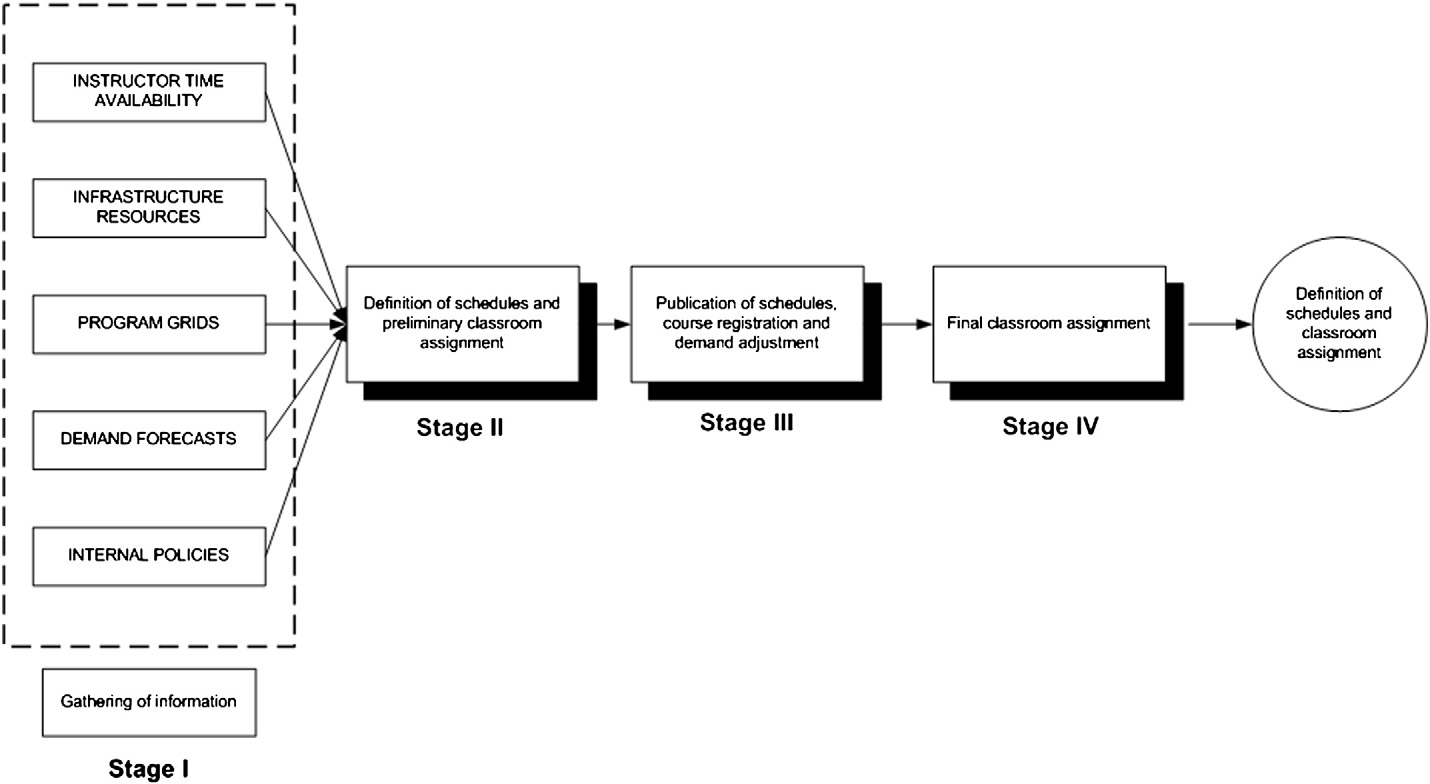
\includegraphics[scale=0.5]{files/img/Arquitetura/Arquitetura-UDP.png}
  \legend{Fonte: \cite{miranda_udpskeduler_2012}}
\end{figure}

Na \autoref{fig:geral}, estão dispostos 4 estágios principais. O primeiro dispõe da aquisição de informações. O meio de aquisição não é relevante para o momento atual, apenas considera-se que esta informação será obtida. No segundo estágios são definidas grades horárias preliminares para se atribuir os alunos. No terceiro, os alunos se inscrevem e a demanda é ajustada, por fim, no quarto estágio, ocorre a alocação final das salas.

\section{Iteração}

Para se alcançar uma alta satisfação por parte dos \textit{stakeholders}, vê-se necessária a constante interação com os mesmos. Para isto, será seguida a estrutura utilizada por \cite{andre_interaction_2018}.

\begin{figure}[htbp]\centering
  \caption{\label{fig:IxD} Etapas do Design de Interação}
  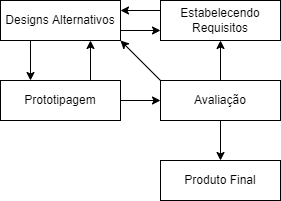
\includegraphics[scale=1]{files/img/Arquitetura/Arquitetura-IxD.png}
  \legend{\selfAuthor}
\end{figure}    % University

Seguindo o conceito do Design de Interação, a \autoref{fig:IxD} ilustra o ciclo de ações a serem tomadas durante o desenvolvimento do sistema, caso este venha a ser necessário. Neste modelo de pesquisa, os \textit{stakeholders} serão consultados continuamente enquanto lhes é apresentado protótipos do sistema, para que assim informem quanto às suas percepções. Esta dinâmica tem como finalidade encontrar um design tal que seja adequado aos desejos e necessidades de seus usuários finais.

\section{Funcionamento}

O sistema final seguirá uma dinâmica similar à que foi ilustrada por \cite{bebis_information_2019} em seu trabalho sobre o uso da Visualização de Informações em relação às Ed-TTPs.

\begin{figure}[htbp]\centering
  \caption{\label{fig:sistema} Funcionamento geral do sistema}
  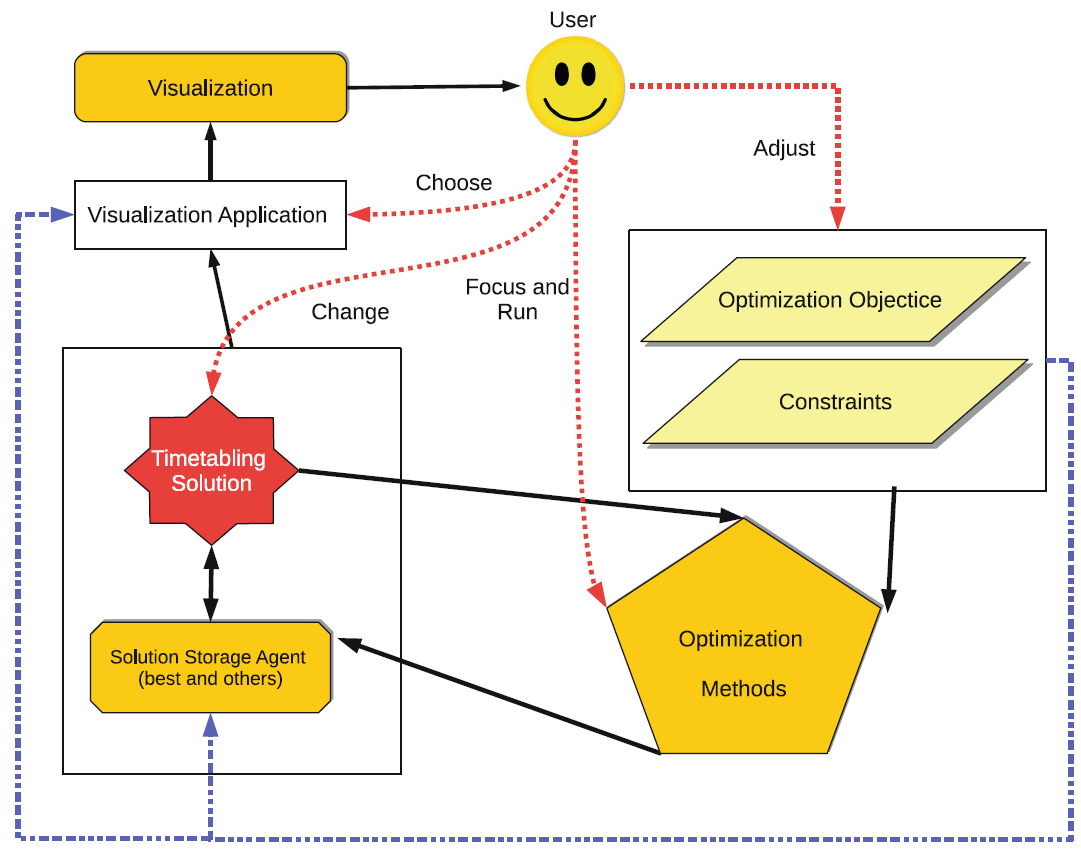
\includegraphics[scale=0.6]{files/img/Arquitetura/Arquitetura_bebis_information_2019.png}
  \legend{Fonte: \cite{bebis_information_2019}}
\end{figure}

A \autoref{fig:sistema} apresenta o comportamento geral do sistema, como seus diferentes segmentos interagem entre si e de que forma o usuário interage com o mesmo. O usuário poderá ajustar os objetivos da otimização e suas restrições, elas serão utilizadas nos métodos de otimização. Estes métodos serão utilizados para se alcançar soluções para estes critérios, as melhores serão então armazenadas. Em posso destes dados, a aplicação apresentará visualmente estas informações ao usuário, permitindo que ele interaja dinamicamente a fim de alcançar seus objetivos.

\section{Modelo de Banco de Dados} \label{ModelagemBD} % ### 5.4. Modelo de Banco de Dados

Considerando as informações necessárias para o presente trabalho, e também o preparo de campo para potenciais aplicações futuras, foi elaborado um diagrama conceitual de banco de dados, que pode ser visto na \autoref{fig:DiagramConceitual}.

\begin{figure}[htbp]\centering
  \caption{\label{fig:DiagramConceitual} Diagrama Conceitual do banco de dados}
  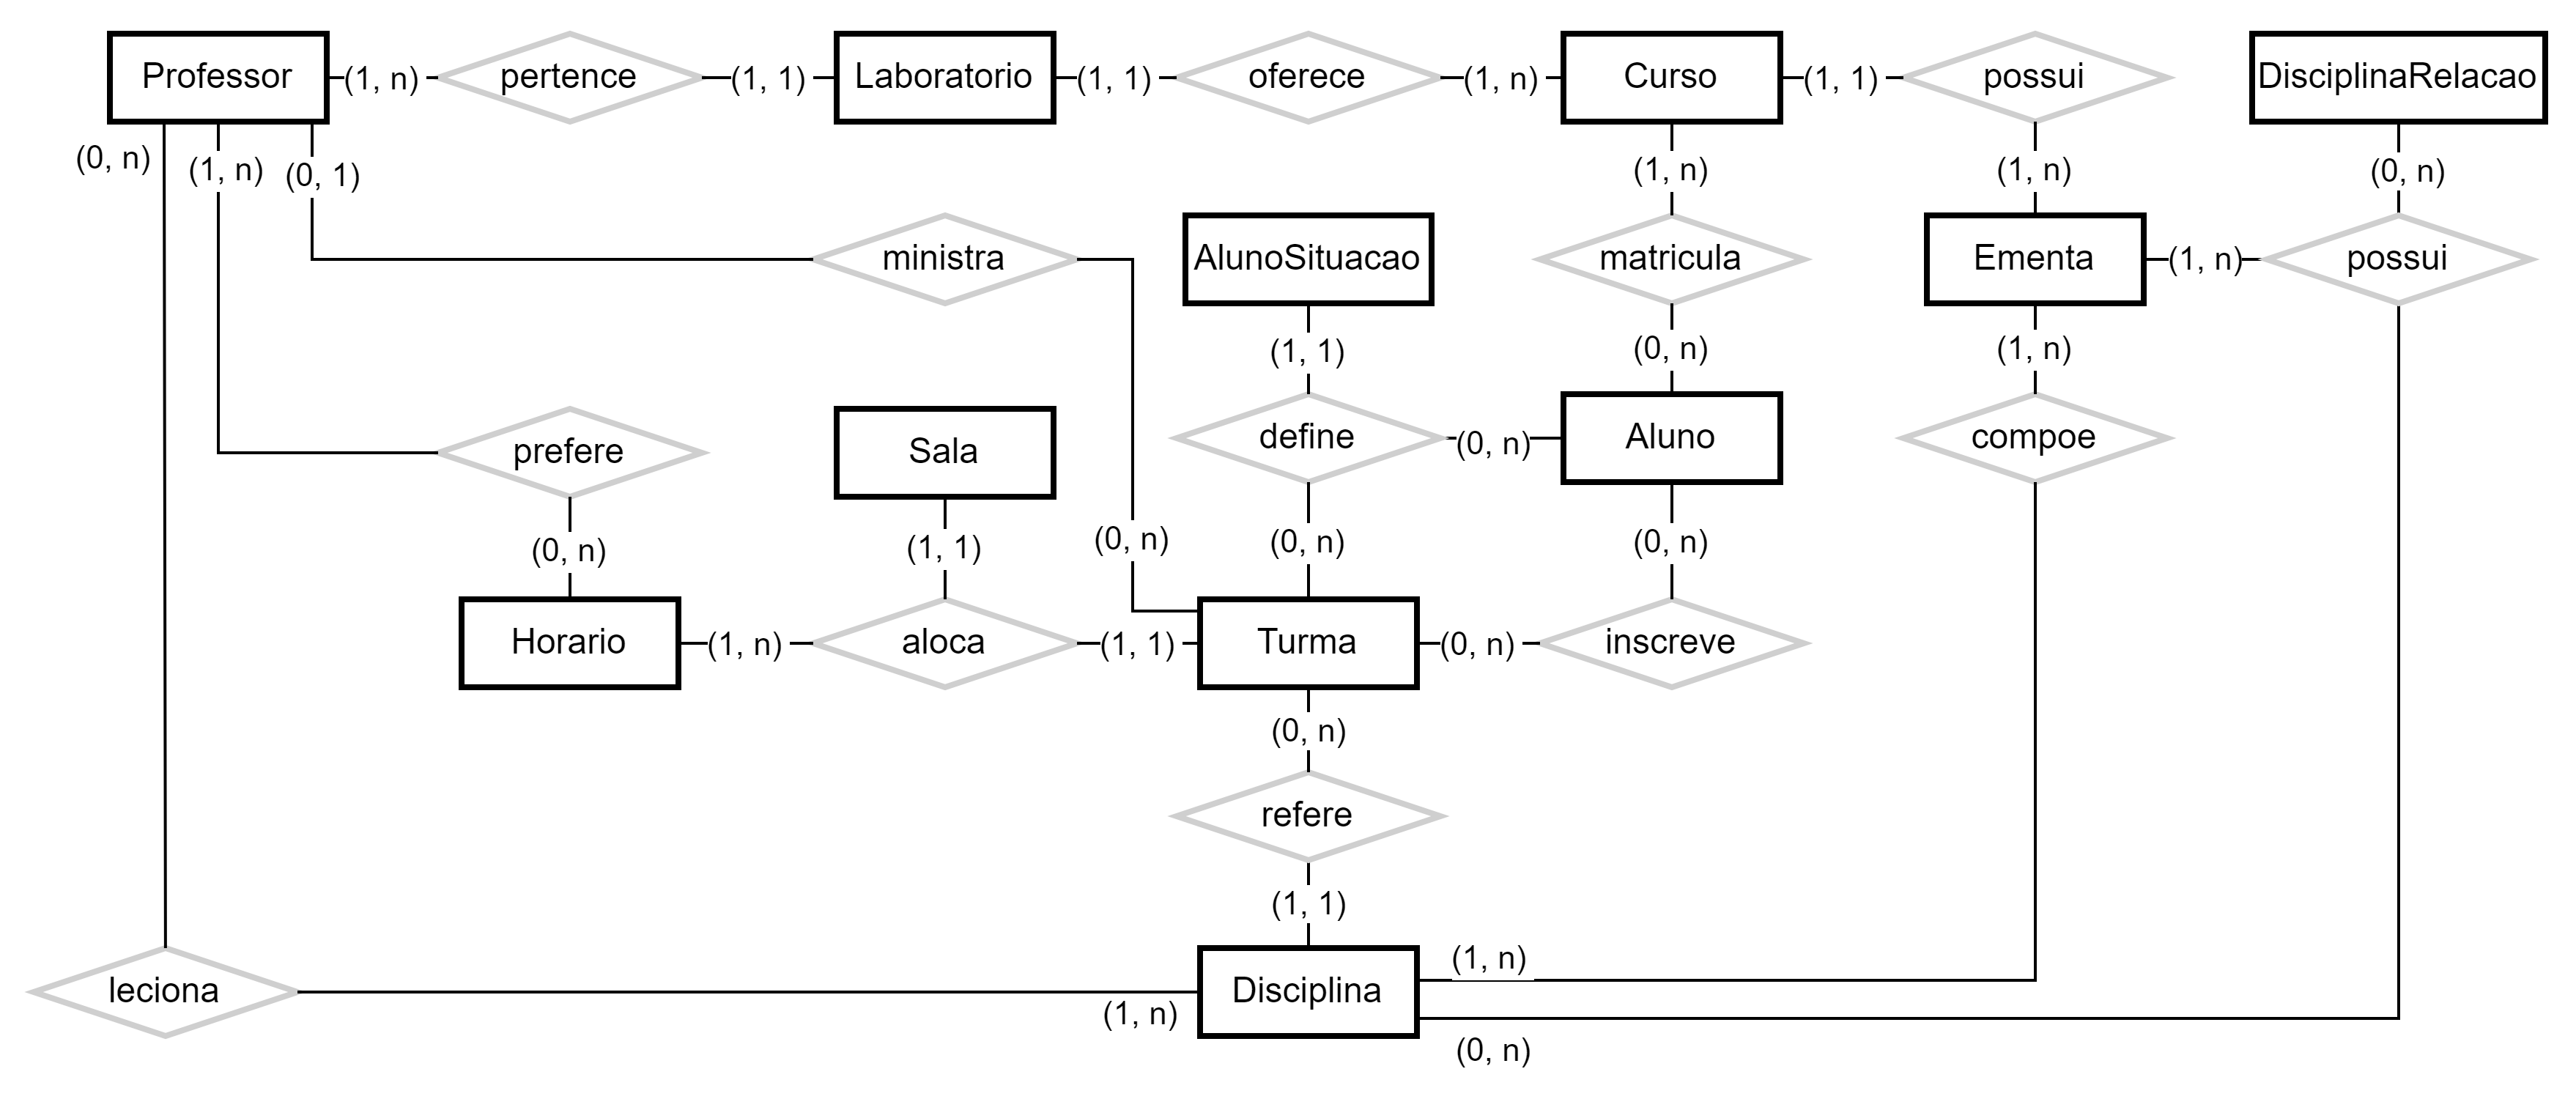
\includegraphics[scale=0.2]{files/img/DiagramaConceitual/DiagramaConceitualBranco.png}
  \legend{\selfAuthor}
\end{figure} % Diagrama Conceitual

O diagrama conceitual foi elaborado utilizando a ferramenta \href{https://www.drawio.com/}{draw.io} citada na metodologia e ilustra as relações entre diversas entidades presentes na realidade da UENF. O emaranhamento presente no diagrama ilustra a complexidade envolvida na criação de uma grade horária, onde diversas entidades se relacionam entre si.

Como principais apontamentos, podemos citar a parte principal do modelo que é a alocação de turmas. Ela, como já descrito, envolve a correlação entre alunos de diferentes cursos, professores, disciplinas, salas e horários. Além disso, também é possível notar a presença de entidades que não são diretamente relacionadas à alocação de turmas, mas que podem se mostrar úteis, como a relação entre professores e laboratórios, e a de disciplinas e ementas.

Embora o diagrama apresente uma visão mais completa de todas as interconexões possíveis, é importante ressaltar que o presente trabalho foca primordialmente na alocação das turmas para o curso de Ciência da Computação, e que a implementação do banco de dados será feita de forma a atender a essas necessidades, fazendo então uso de uma parte do diagrama conceitual.

% Tendo isso em vista, o modelo conceitual reduzido para o presente trabalho pode ser visto na \autoref{fig:DiagramConceitualReduzido}.

% \begin{figure}[htbp]\centering
%   \caption{\label{fig:DiagramConceitualReduzido} Diagrama Conceitual reduzido para o presente trabalho}
%   \includegraphics[scale=0.2]{files/img/DiagramaConceitual/DiagramaConceitualReduzidoBranco.png}
%   \legend{\selfAuthor}
% \end{figure} % Diagrama Conceitual reduzido

Neste modelo, mais enxuto, temos apenas as entidades principais, onde temos uma turma de determinada disciplina, ministrada por um professor e que ocorre em uma sala em um determinado horário.

\subsection{Diagrama de Entidade e relacionamento} % ### 5.4.1. Modelo Relacional

% Com isso, restamos o diagrama de Entidade e Relacionamento (DER) que pode ser visto na \autoref{fig:DER}.

% \begin{figure}[htbp]\centering
%   \caption{\label{fig:DER} Diagrama de Entidade e Relacionamento}
%   \includegraphics[scale=0.2]{files/img/DER/DERBranco.png}
%   \legend{\selfAuthor}
% \end{figure} % Diagrama de Entidade e Relacionamento

Neste diagrama vemos as entidades principais, que são \textit{Turmas}, \textit{Disciplinas}, \textit{Professores}, \textit{Horários} e \textit{Salas}. As propriedades escolhidas para cada entidade são compostas por uma mistura de critérios. Por exemplo, o nome do professor, o código da disciplina, e a junção de código e bloco auxiliam primordialmente na identificação real dos professores, disciplinas e salas. Já as informações ``período'', ``apelido'' e ``comment''...

E também é notável a presença da entidade \textit{Alunos}, que se apresenta desacoplado das demais entidades. O motivo para isso é que, embora os alunos façam parte do processo de alocação de turmas, ao longo do desenvolvimento, o desenvolvimento de funcionalidades envolvendo os alunos...
